\documentclass[tikz,12pt]{standalone}
\usetikzlibrary{arrows,angles,quotes}% tikz package already loaded by 'tikz' option
\begin{document}
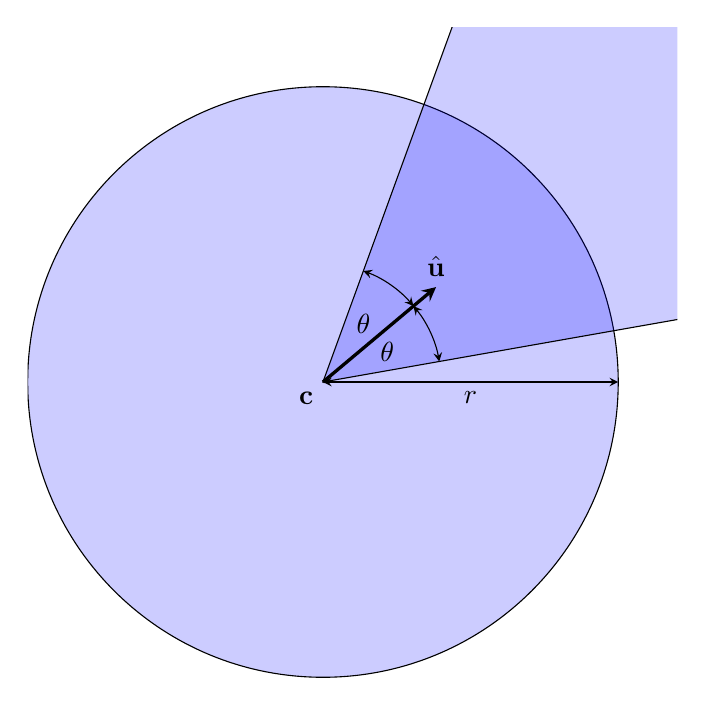
\begin{tikzpicture}[scale=0.75,>=stealth]
  \newcommand*{\Radius}{5cm}
  \newcommand*{\RadiusLong}{10cm}
  \newcommand*{\Direction}{40}
  \newcommand*{\Angle}{30}
  \coordinate (A) at (\Direction - \Angle:\RadiusLong);
  \coordinate (O) at (0,0);
  \coordinate (B) at (\Direction + \Angle:\RadiusLong);
  \coordinate (U) at (\Direction:\Radius * 0.5);
  \clip (-\Radius, -\Radius) rectangle(1.2 * \Radius, 1.2 * \Radius);
  \filldraw[fill=blue!20] (O) circle[radius=\Radius];
  \draw (A) -- (O) -- (B) pic [fill=blue,opacity=0.2, angle radius=\RadiusLong] {angle = A--O--B};
  \draw (O) node[anchor=north east] {$\mathbf{c}$};
  \draw[<->] (O) -- (0:\Radius) node[midway, anchor=north] {$r$};
  \draw pic [draw=black, <->, angle radius=1.5cm, "$\theta$"] {angle = A--O--U};
  \draw pic [draw=black, <->, angle radius=1.5cm, "$\theta$"] {angle = U--O--B};
  \draw[->, very thick] (O) -- (U) node[anchor=south] {$\hat\mathbf{u}$}; 
\end{tikzpicture}
\end{document}
